\section{First Part (ViolaJones):}
The code for Viola Jones is composed by the following files
\begin{itemize}
	\item \textbf{ConvertHaarcasadeXMLOpenCV.m}: This function is required to translate OpenCV feature functions from XML to syntax Matlab in order to be compiled.
	\item \textbf{ObjectDetection.m}: This is the beginning of the detection, where the input parameters are received and invokes the functions \textbf{GetIntergralImages.m} and  \textbf{HaarCasadeObjectDetection.m}.
	\item \textbf{GetIntergralImages.m}: This function computes the \textbf{integral matrix} for the image.
	\item \textbf{HaarCasadeObjectDetection.m}: This function uses the Cascade Classifier to calculate the \textbf{Rectangle} matrices. 
\end{itemize}

\subsection{Code:}
\noindent Let start by describing what is important about the codes.\\
\noindent The first code called is \textbf{ObjectDetection.m} Listing \ref{lst:ObjectDetection}.\\%xq primero listing2? 
\noindent On line 3 of the Listing \ref{lst:ObjectDetection}, we have the default options:
\begin{itemize}
	\item \textbf{ScaleUpdate}: This tells us that the scale of the current \textbf{window} will increase from 1 to 1.2 in each iteration. Thus, if the current scale is $X$, the next scale will be $1.2X$. 
	\item \textbf{Resize}: Resizes the image so that the longest side (width or height) is equal to 384.
	\item \textbf{Verbose}: To show the calculations of the iterations.
\end{itemize}

\noindent On line 31 of the Listing \ref{lst:ObjectDetection}, we load the image and convert it into an array, but if the image is coloured then the pixels of the array has 3 values in each pixel $(r,g,v)$.\\

\noindent On line 35 of the Listing \ref{lst:ObjectDetection}, this function extracts the feature functions already trained by \textbf{OpenCV}, which are our \textbf{Strong Classifiers} when examining each \textbf{window}, as shown in lecture slide in Figure \ref{fig:slideT1}.\\

\noindent On line 37 of the Listing \ref{lst:ObjectDetection},we compute the \textbf{integral matrix} using the function \textbf{GetIntergralImages.m} (see Listing \ref{lst:GetIntergralImages}).\\ 

\noindent On line 1 of the Listing \ref{lst:GetIntergralImages}, we convert the image array to a double-type.\\

\noindent On lines from 2 to 12 of the Listing \ref{lst:GetIntergralImages}, the image resize mentioned is performed (option resize). The reason for the ratio between the real size of the image and its current size is saved $Ratio=size(Picture,2)/384$.\\

\noindent On lines from 14 to 16 of the Listing \ref{lst:GetIntergralImages}, we convert the image to greyscale, which means, that our pixels no longer have 3 values (r,g,b) but have a single value.\\

\noindent On lines from 18 to 39 of the Listing \ref{lst:GetIntergralImages}, we compute the \textbf{integral matrix} for the image. In the Figure \ref{fig:integral} we can see how compute the  \textbf{integral matrix}.

\noindent On lines from 41 to 62 of the Listing \ref{lst:GetIntergralImages}, we compute the \textbf{integral matrix} for $I2$, where $I2$ is
\begin{equation}
	\text{let }	I=
	\begin{pmatrix}
		i_{11} & i_{12} & \cdots & i_{1n}\\
		i_{21} & i_{22} & \cdots & i_{2n}\\
		\vdots & \vdots & \ddots & \vdots\\
		i_{m1} & i_{m2} & \cdots & i_{mn}\\
	\end{pmatrix}
	\Rightarrow I2=
	\begin{pmatrix}
		(i_{11})^2 & (i_{12})^2 & \cdots & (i_{1n})^2\\
		(i_{21})^2 & (i_{22})^2 & \cdots & (i_{2n})^2\\
		\vdots & \vdots & \ddots & \vdots\\
		(i_{m1})^2 & (i_{m2})^2 & \cdots & (i_{mn})^{2}\\
	\end{pmatrix}
\end{equation}

\noindent On lines from 64 to 66 of the Listing \ref{lst:GetIntergralImages}, here we only add the \textbf{height} and \textbf{width} of the current image (with a maximum side like 384), and the \textbf{ratio} of change of the image resize to structure $IntegralImages$.\\ %side or size?

\noindent On line 39 of the Listing \ref{lst:ObjectDetection}, we call the function $HaarCasadeObjectDetection$, which applies cascade classification to find the \textbf{Rectangle} matrices that contain the faces that appear in the image.\\

\noindent On line from 1 to 7 of the Listing \ref{lst:HaarCasadeObjectDetection}, we calculate the initial window size.\\

\noindent On line 11 of the Listing \ref{lst:HaarCasadeObjectDetection}, we calculate the number of total iterations, that is, the number of different \textbf{window} sizes that exist with the $Options.ScaleUpdate$.\\

\noindent On line from 13 to 35 of the Listing \ref{lst:HaarCasadeObjectDetection}, we compute the \textbf{Rectangle} matrices using the properties of the \textbf{integral matrix} \ref{fig:integral_properties}.\\

\noindent On line 9 of the Listing \ref{lst:HaarCasadeObjectDetection}, we transform the \textbf{Rectangle} matrices to the original size of the image.

\begin{figure}[h!]
	\centering
	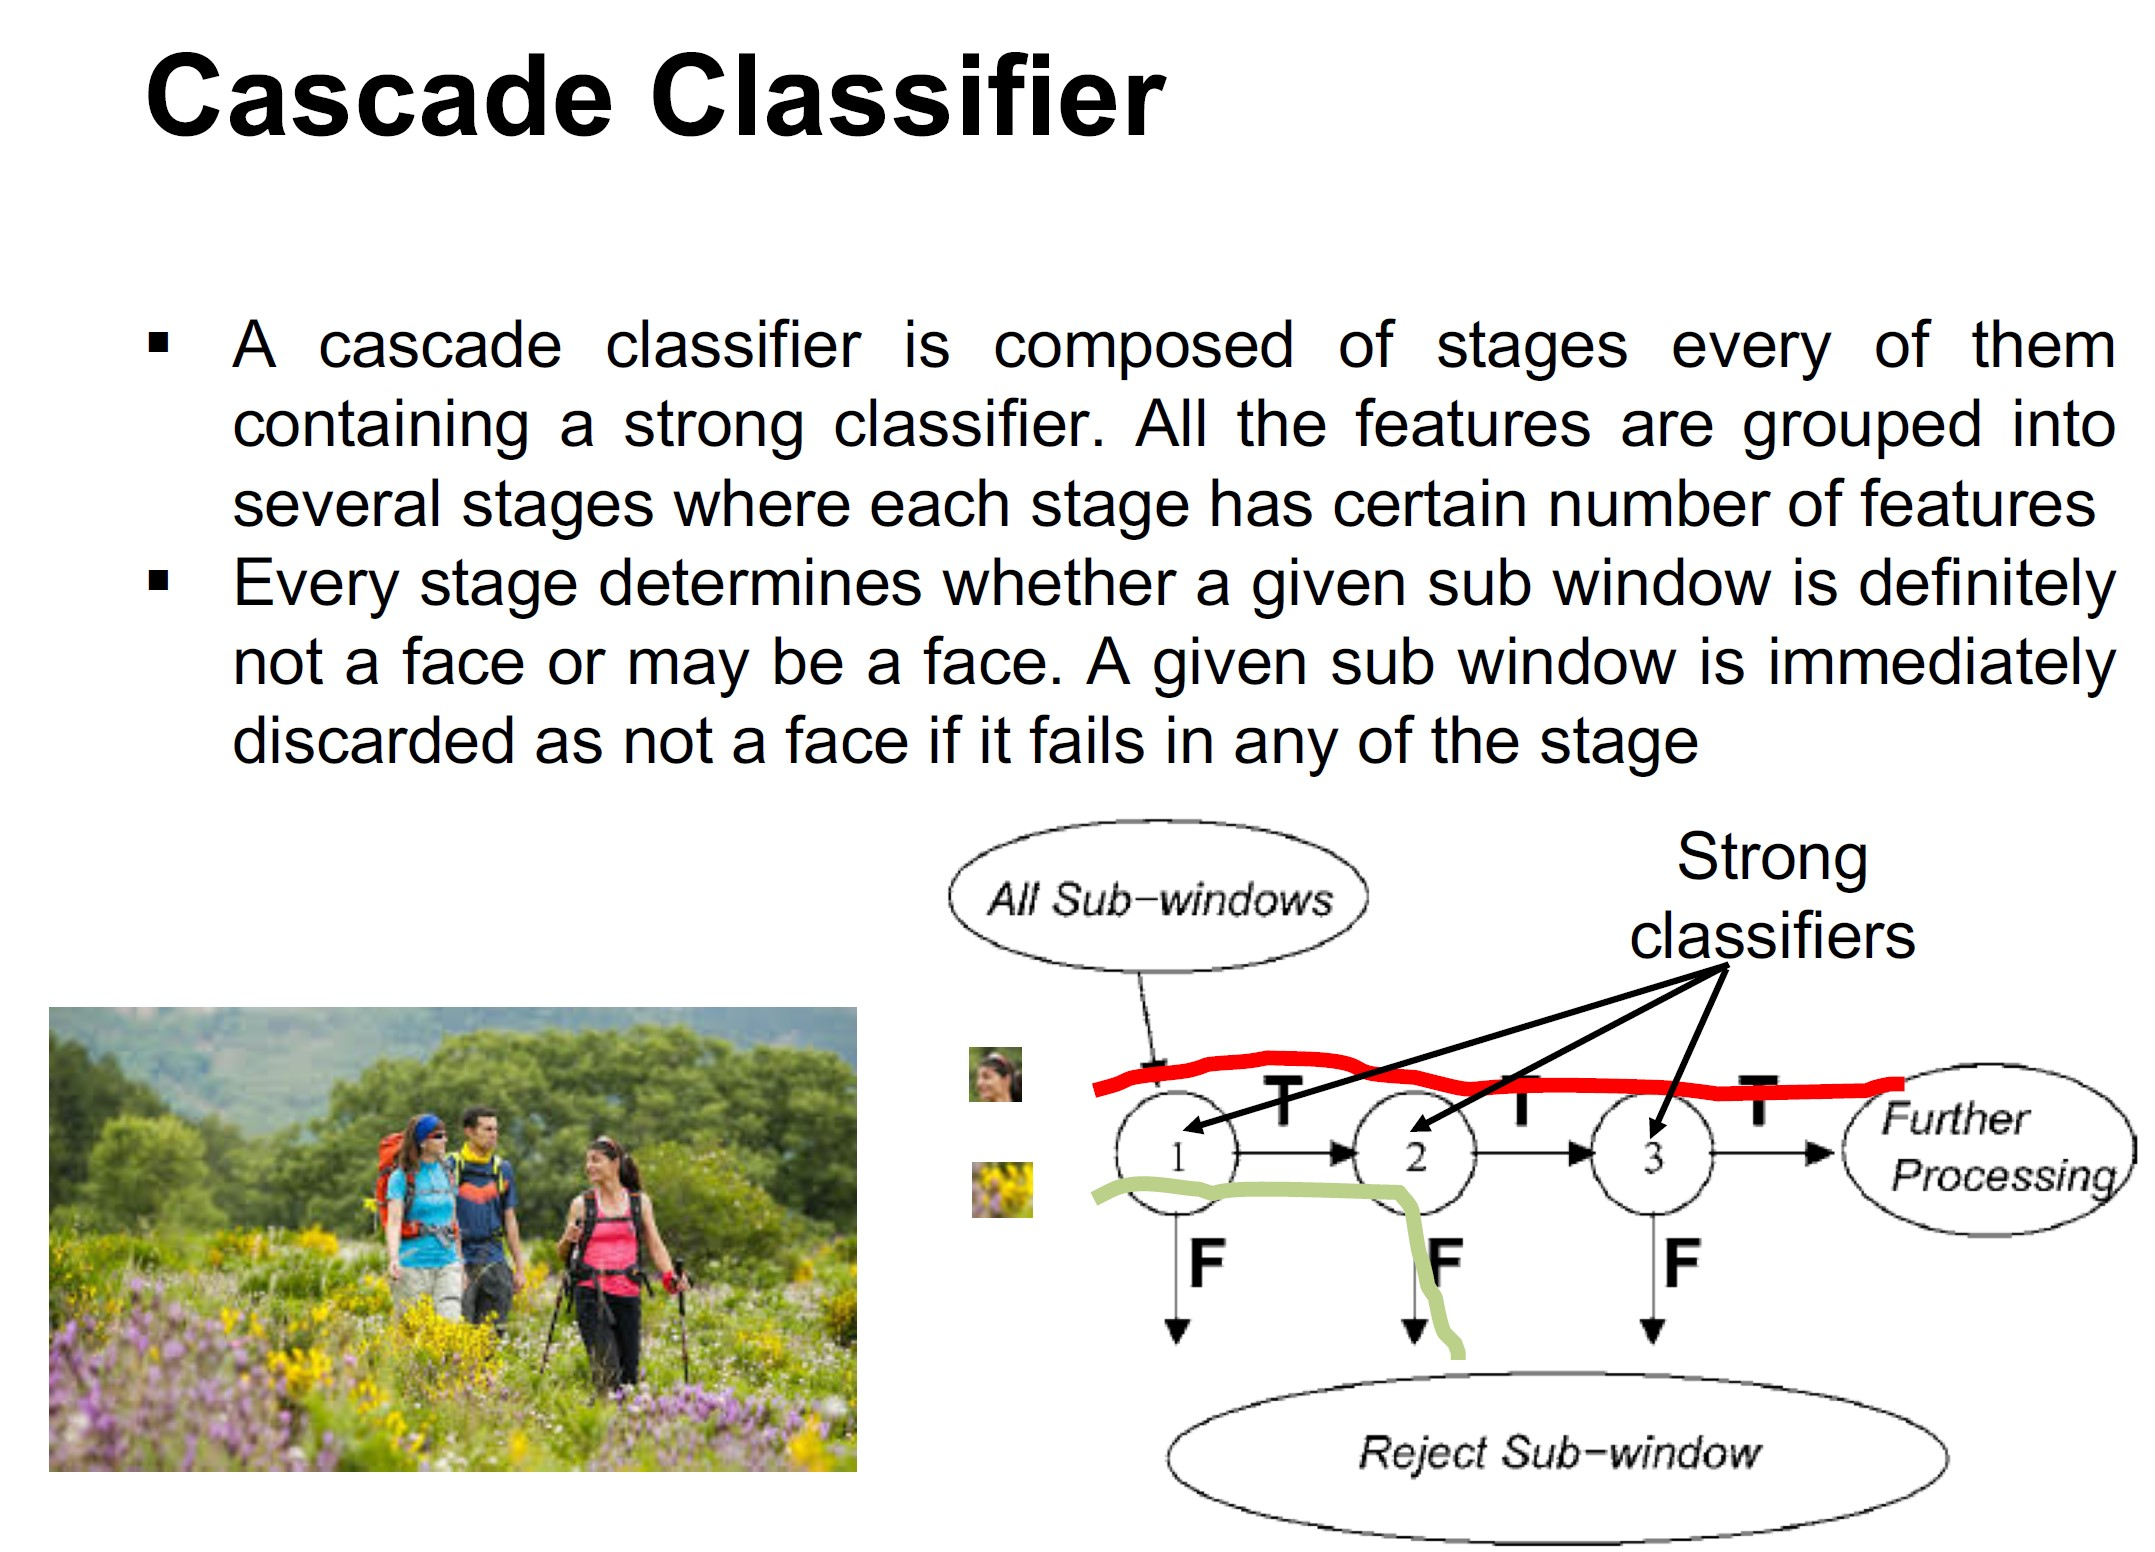
\includegraphics[width=0.65\textwidth]{T1/classifier}
	\caption{Cascade Classifier}
	\label{fig:slideT1}
\end{figure}
\begin{figure}[h!]
	\centering
	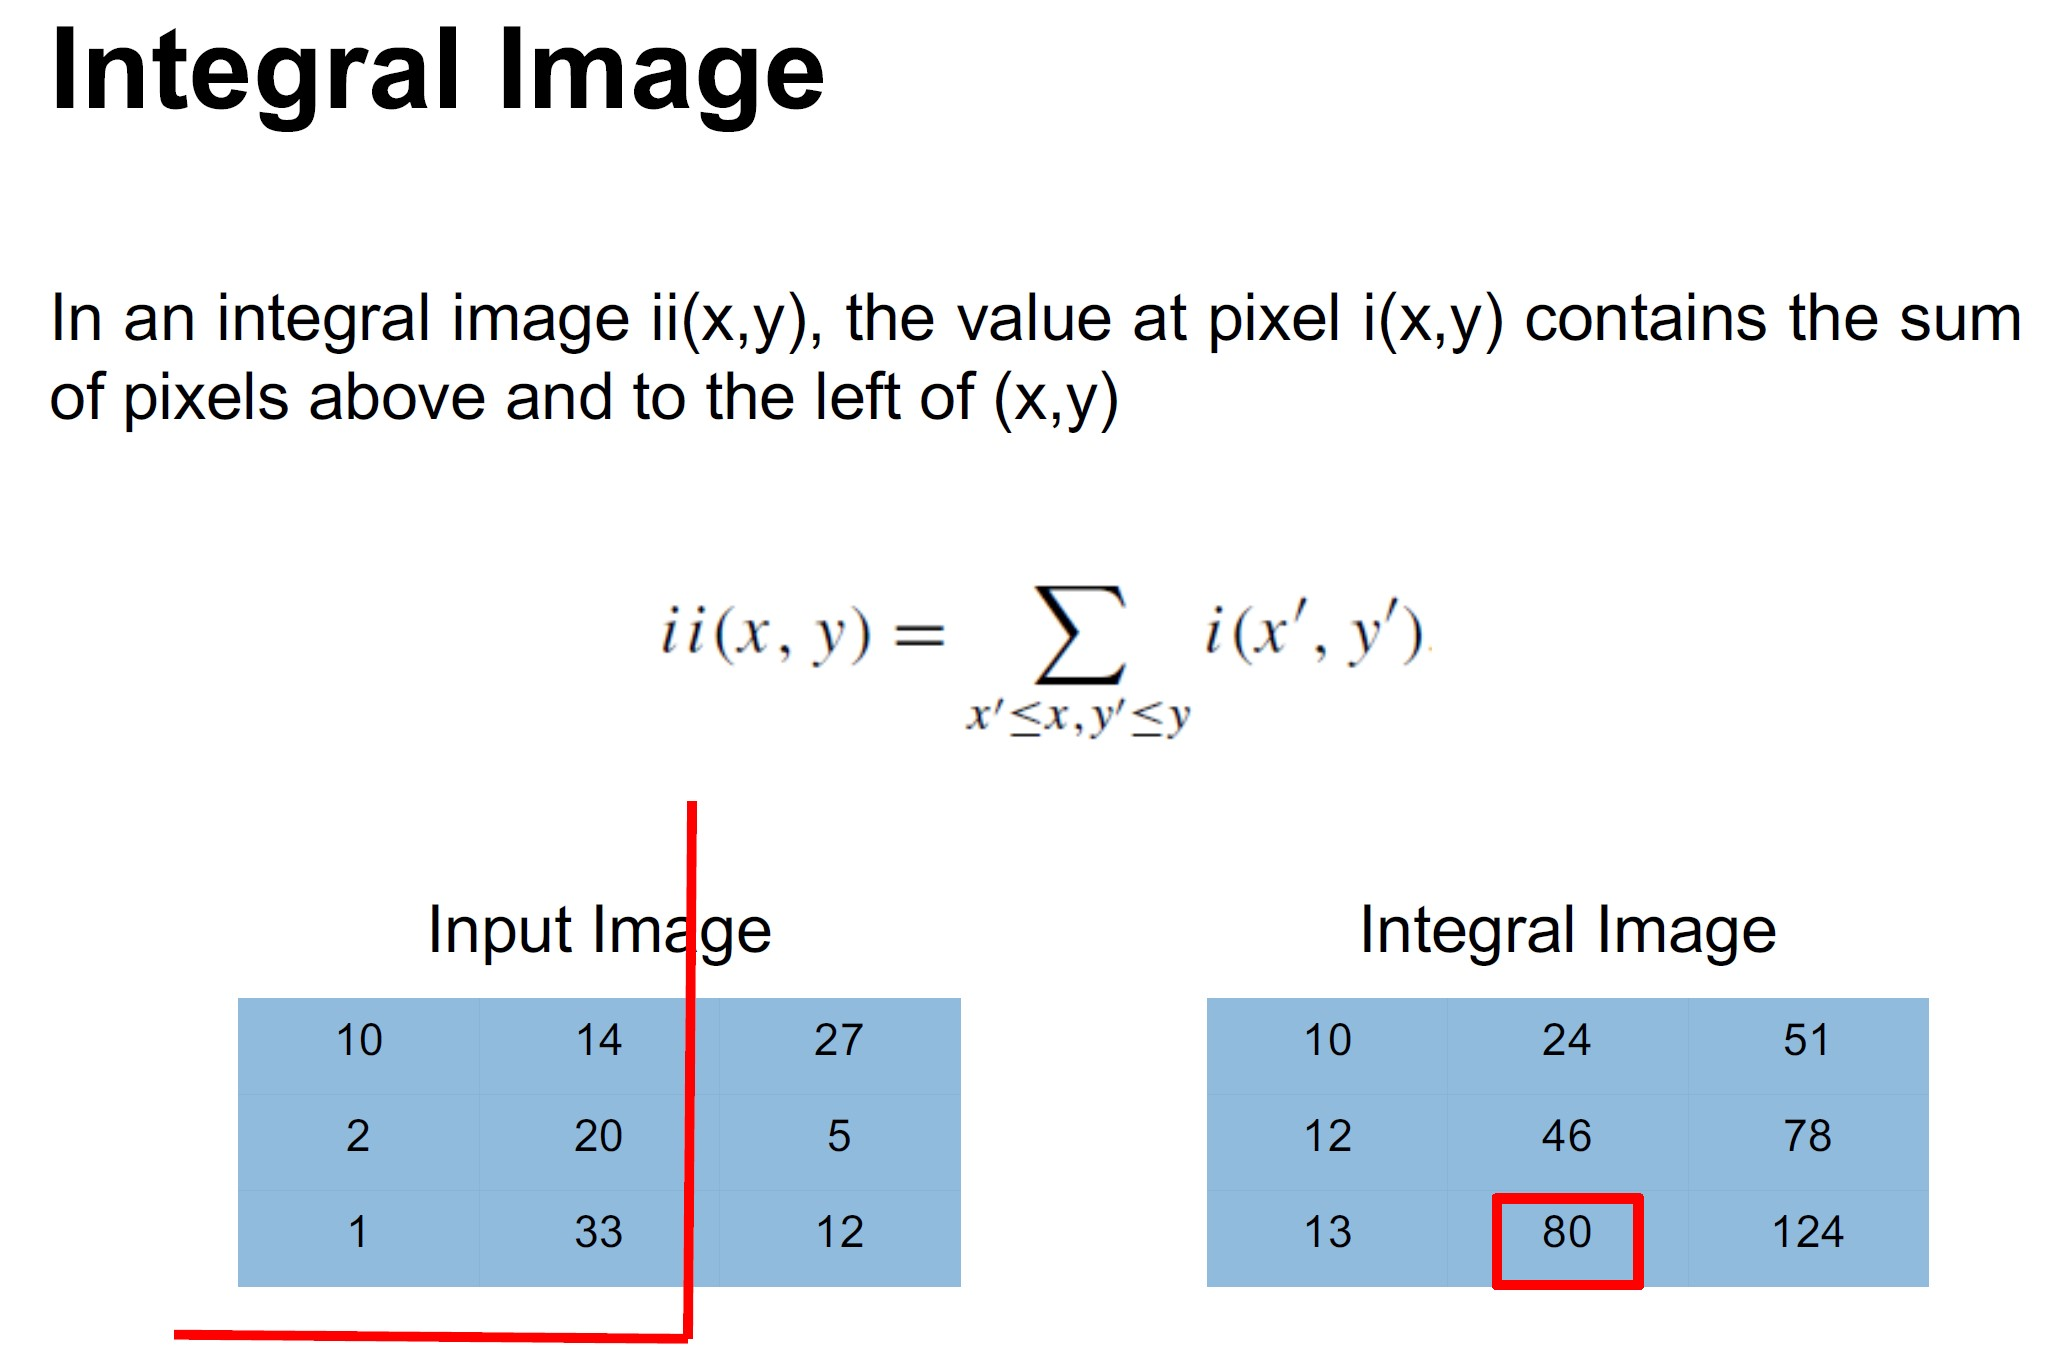
\includegraphics[width=0.65\textwidth]{T1/integral_image}
	\caption{Integral Image calculation}
	\label{fig:integral}
\end{figure}
\begin{figure}[h!]
	\centering
	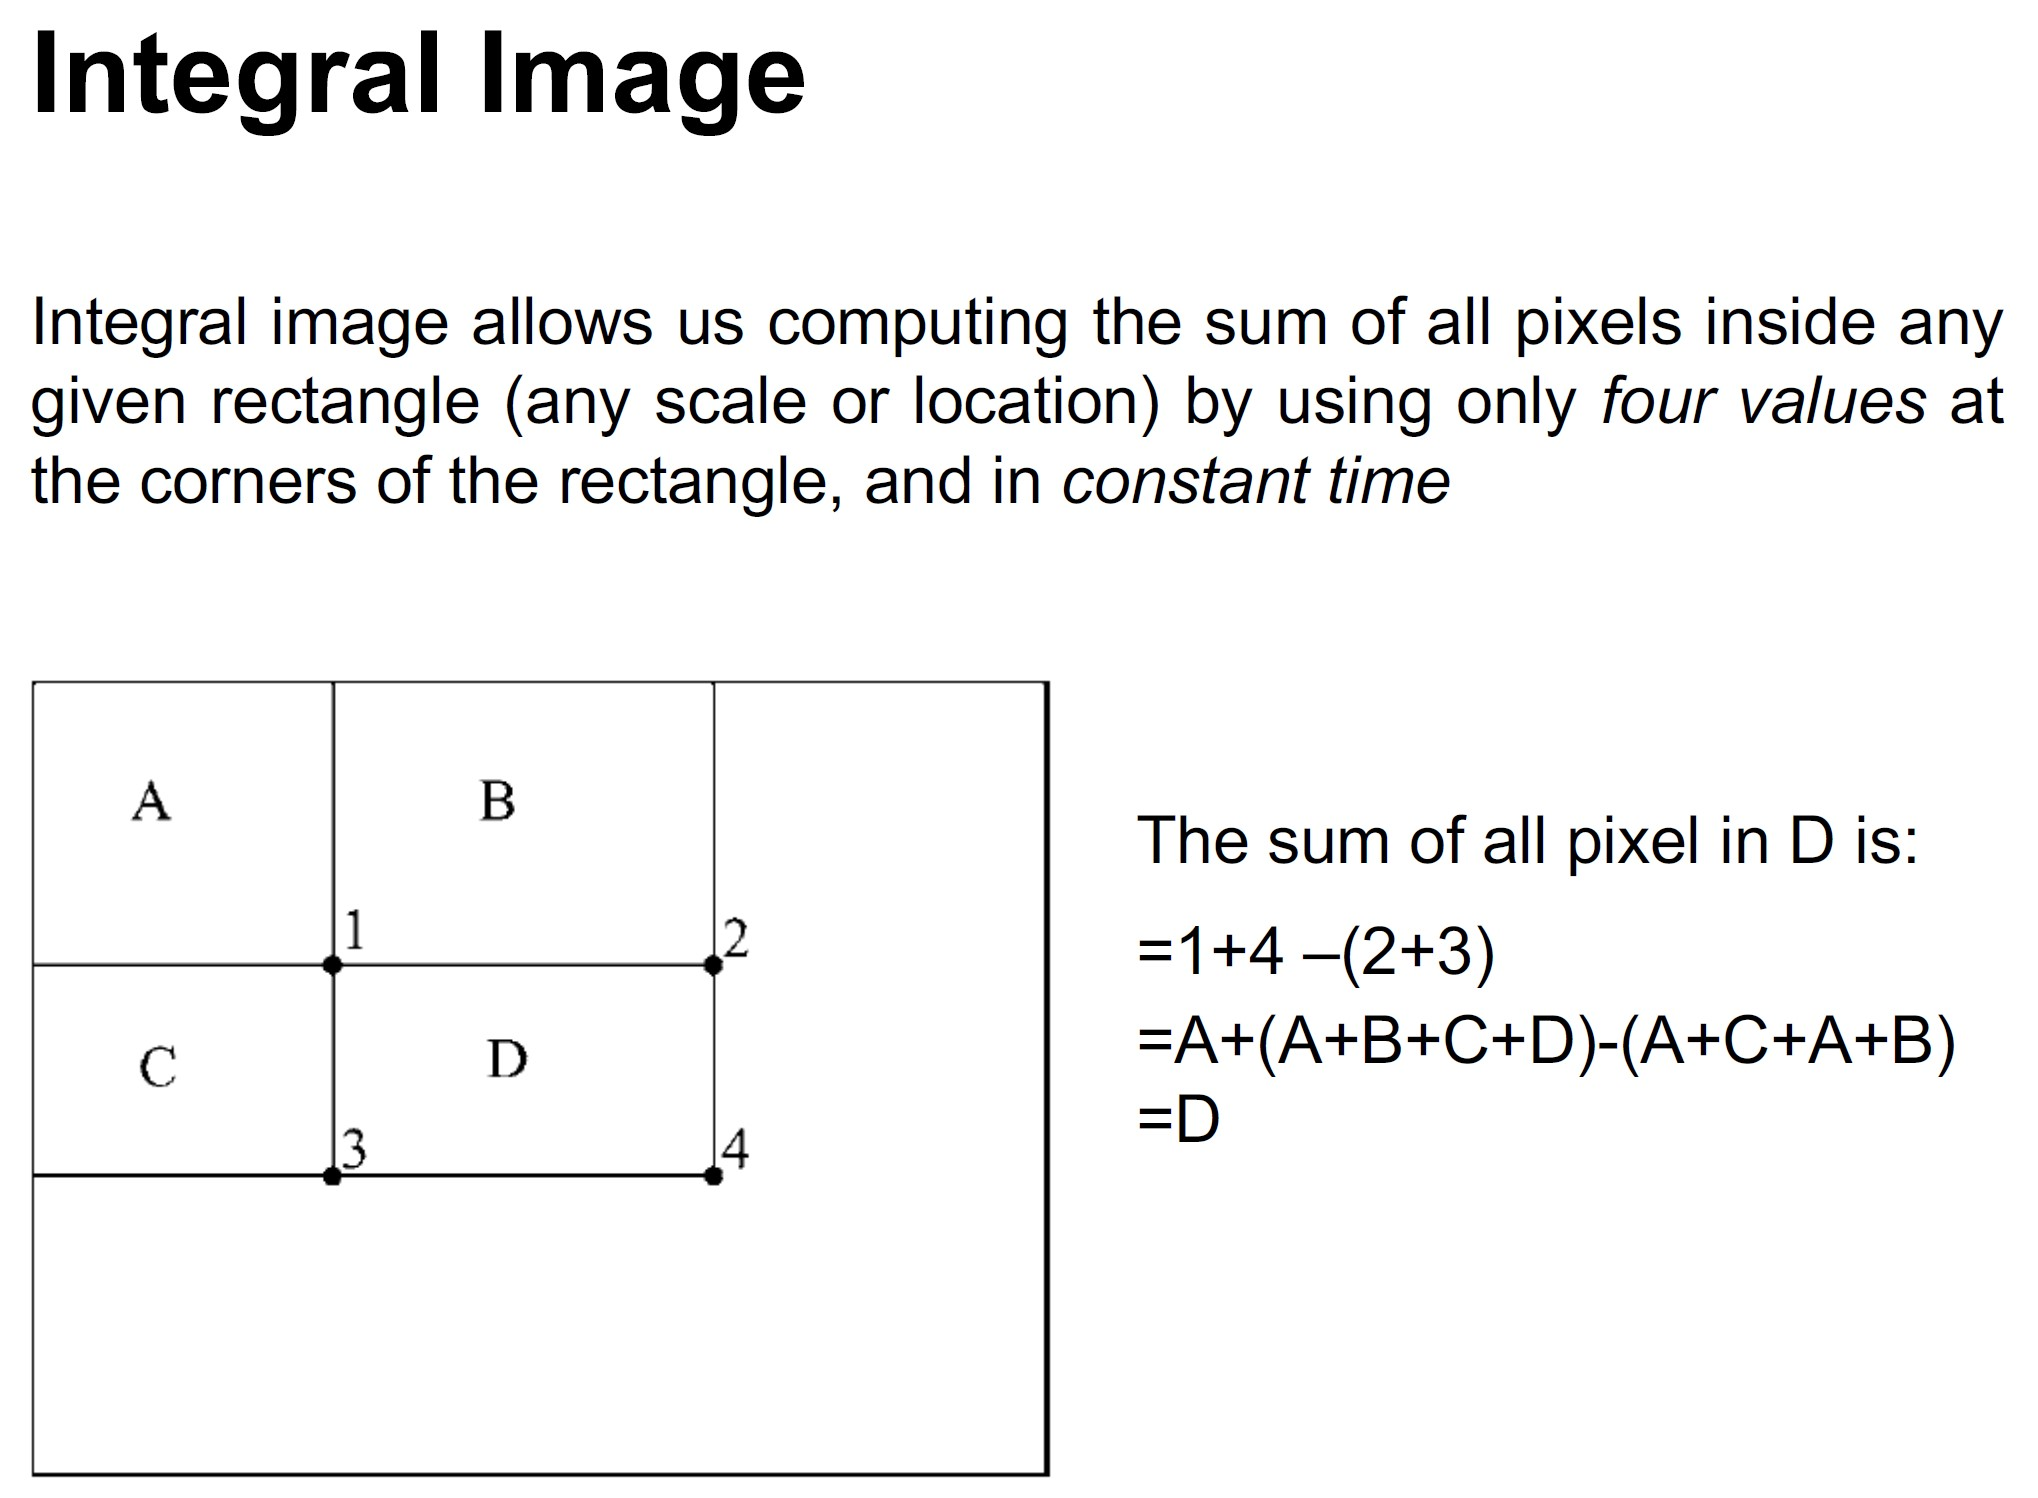
\includegraphics[width=0.65\textwidth]{T1/integral_image_properties}
	\caption{Integral Image properties}
	\label{fig:integral_properties}
\end{figure}

\subsection{Results:}

\noindent Here we show an image where some faces are clearly visible, which are enclosed in the \textbf{Rectangles} that can be seen in Figure \ref{fig:image}.\\


\begin{figure}[h!]
	\centering
	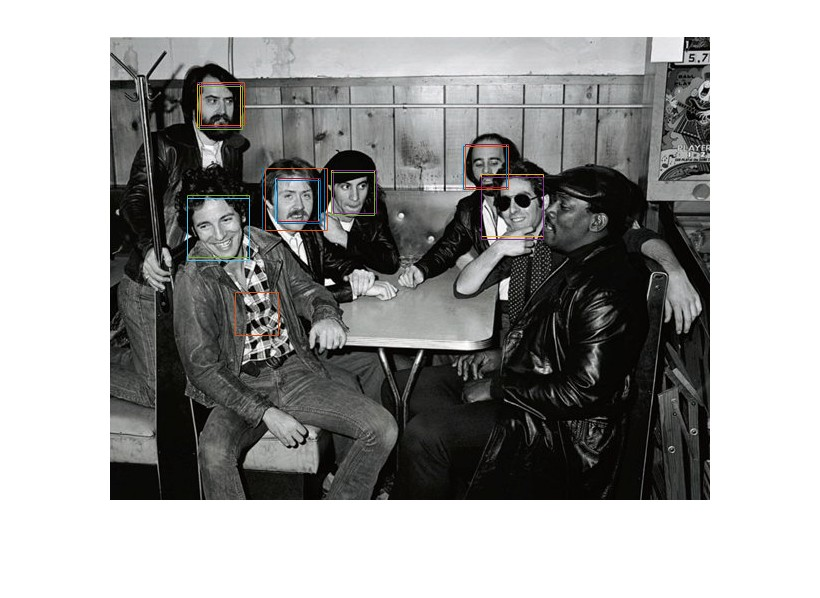
\includegraphics[width=0.65\textwidth]{T1/image}
	\caption{This image contains the detected \textbf{Rectangle}}
	\label{fig:image}
\end{figure}
\noindent And in figure \ref{fig:scale} we can see how many faces were found per scale.
\begin{figure}[h!]
	\centering
	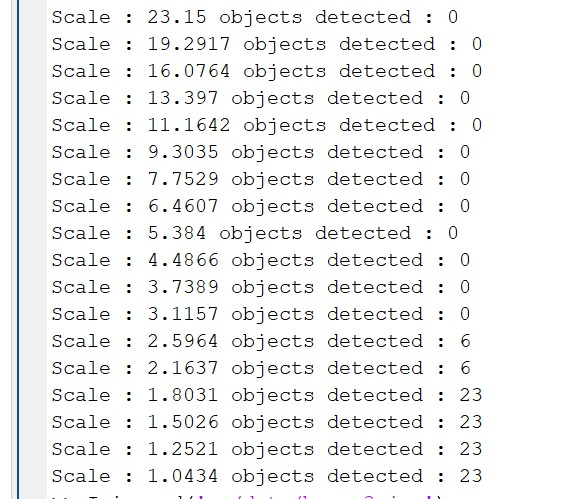
\includegraphics[width=0.60\textwidth]{T1/scales}
	\caption{These are the \textbf{Rectangle} found in each scale}
	\label{fig:scale}
\end{figure}